\documentclass[a4paper,10pt]{article}
\usepackage{graphicx} 
\usepackage[utf8]{inputenc}
\usepackage[spanish]{babel}
\usepackage{fancyhdr}
\usepackage{multicol}
\usepackage{geometry}
\usepackage{listings}
\usepackage{xcolor}
\geometry{a4paper, portrait, margin=1in}

\pagestyle{fancy}
\fancyhf{}
\fancyhead[L]{\textbf{Métodos de Optimización}}
\fancyhead[R]{Universidad Nacional del Altiplano - FINESI}
\fancyfoot[C]{\thepage}

\begin{document}

\title{\textbf{  Resolución de Sistemas de Ecuaciones Lineales\\ Python, R con Shiny}}
\author{
  NOMBRE: Beatriz Umiña Machaca\\
  Código: 230035 \\
  Docente: Fred Torres Cruz
}
\date{05 de mayo de 2025}

\maketitle
\thispagestyle{fancy}  


\section*{1. Introducción}

El propósito de este proyecto es resolver sistemas de ecuaciones lineales con dos variables (x y y) utilizando métodos algebraicos: \textbf{sustitución}, \textbf{igualación} y \textbf{reducción}. El sistema fue inicialmente implementado en \textbf{Python} para su uso en consola, y posteriormente migrado y mejorado en \textbf{R} utilizando el paquete \textit{Shiny}, para ofrecer una interfaz gráfica interactiva.

\section*{2. Primera Versión: Python (Interfaz de Consola)}

\subsection*{Características}

\begin{itemize}
    \item Implementación en consola usando \texttt{sympy}, \texttt{re} y entrada de texto con \texttt{input()}.
    \item Análisis de ecuaciones con expresiones regulares (\texttt{re.match}).
    \item Resolución de sistemas mediante tres métodos:


\begin{center}
    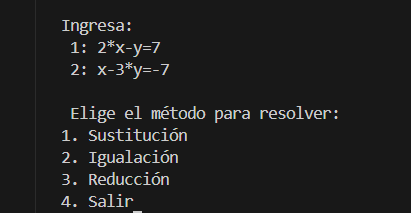
\includegraphics[width=0.6\textwidth]{imagen_metodos.png} 
\end{center}
    
    \begin{itemize}
        \item Sustitución
        
        \begin{center}
            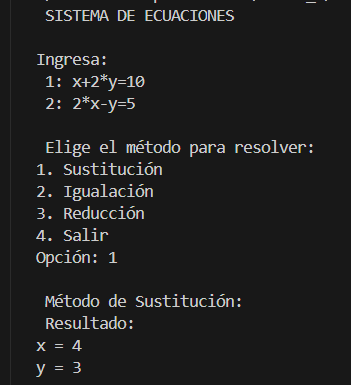
\includegraphics[width=0.6\textwidth]{sustitucion.png}
        \end{center}
        
        \item Igualación
        
        \begin{center}
            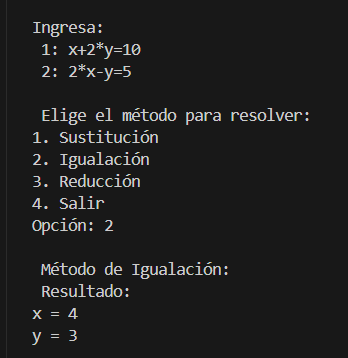
\includegraphics[width=0.6\textwidth]{igualacion.png}
        \end{center}
        
        \item Reducción (resolución directa con \texttt{solve})
        
        \begin{center}
            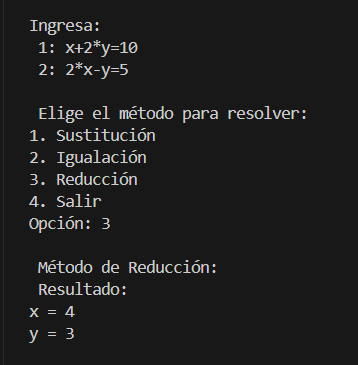
\includegraphics[width=0.6\textwidth]{reduccion.png}
        \end{center}
    \end{itemize}
    \item Manejo de errores en entrada y resolución.
\end{itemize}


\subsection*{Lógica de resolución}

\begin{itemize}
    \item Se parsean ecuaciones tipo \texttt{ax + by = c} desde texto.
    \item Se despeja una variable y se sustituye en la otra ecuación.
    \item Se imprime el resultado paso a paso para el usuario.
\end{itemize}

\subsection*{Ventajas}
\begin{itemize}
    \item Rápido de desarrollar.
    \item Ideal para pruebas de lógica algebraica.
\end{itemize}

\subsection*{Limitaciones}
\begin{itemize}
    \item Requiere conocimiento básico de sintaxis matemática para ingresar las ecuaciones.
    \item No amigable para usuarios no técnicos.
    \item Poco visual e interacción limitada.
\end{itemize}

\section*{3. Segunda Versión: R con Shiny (Interfaz Gráfica Web)}

\subsection*{Características}

\begin{itemize}
    \item Interfaz gráfica desarrollada con \texttt{shiny}, accesible vía navegador.

    \item[] \href{http://127.0.0.1:6597}{\textcolor{blue}
    \begin{center}
        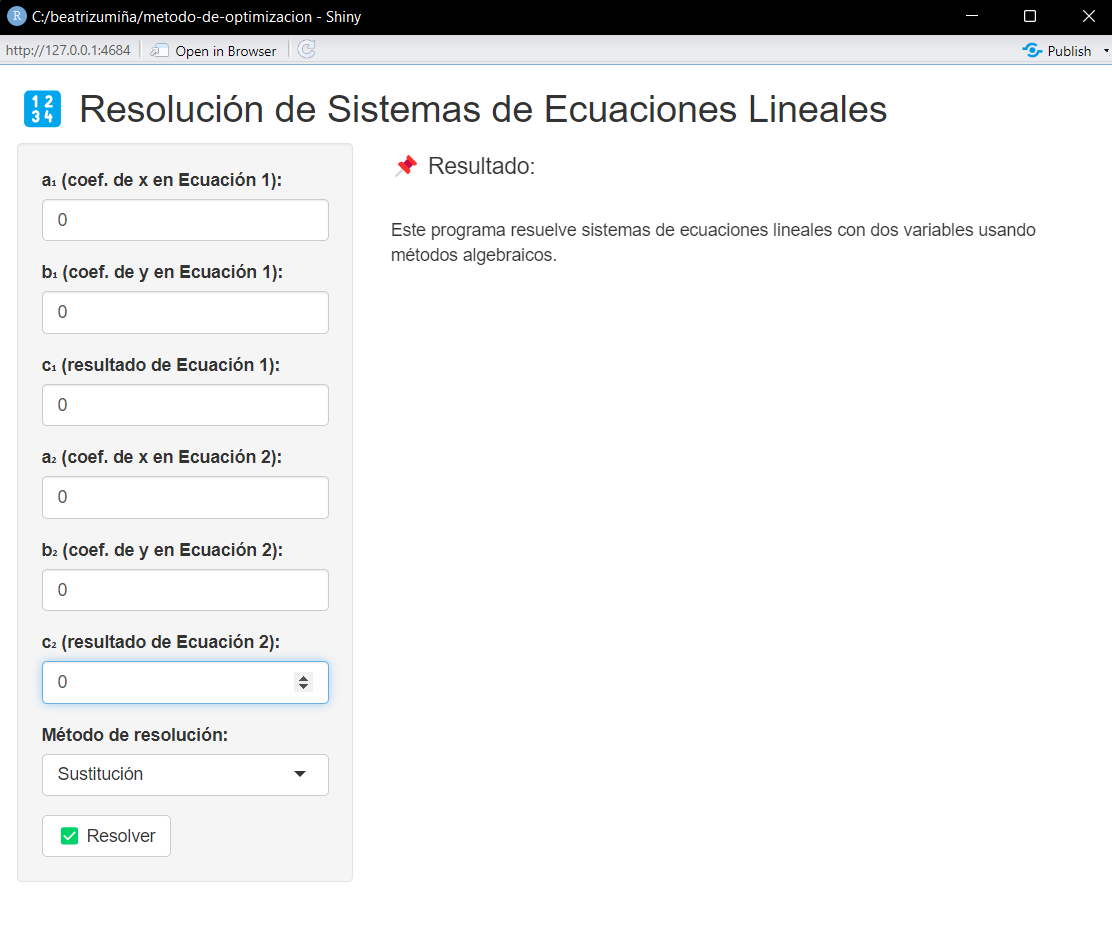
\includegraphics[width=0.5\textwidth]{interfaz_shiny.png} 
    \end{center}
    
    \item Entradas numéricas para coeficientes \texttt{a}, \texttt{b}, \texttt{c} de cada ecuación.
    \begin{center}
        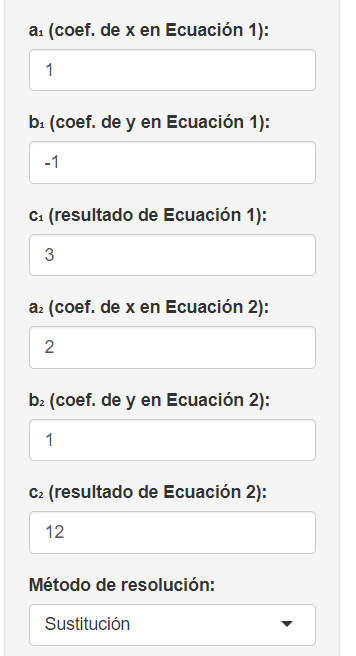
\includegraphics[width=0.5\textwidth]{entradas_coeficientes.png} 
    \end{center}
    
    \item Menú desplegable para elegir el método de resolución.
    \begin{center}
        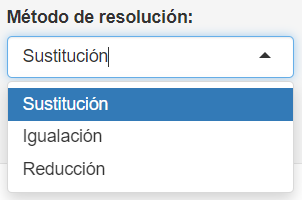
\includegraphics[width=0.5\textwidth]{menu_metodo.png} 
    \end{center}
    
    \item Botón para ejecutar el cálculo y mostrar resultados.
    \begin{center}
        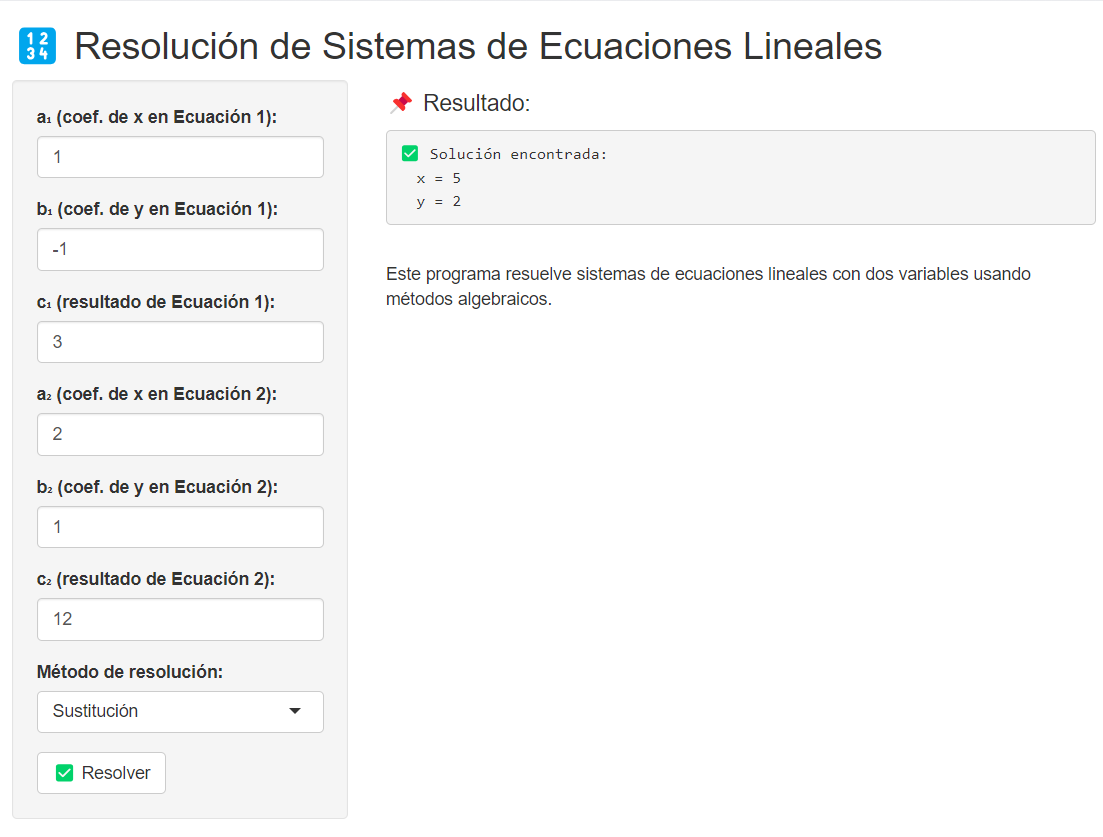
\includegraphics[width=0.5\textwidth]{boton_calcular.png} 
    \end{center}
\end{itemize}


\subsection*{Lógica de resolución}

\begin{itemize}
    \item Los métodos implementan la lógica matemática directamente en R:
    \begin{itemize}
        \item En sustitución e igualación, se usan funciones y \texttt{uniroot} para encontrar raíces.
        \item En reducción, se resuelve el sistema con álgebra matricial (\texttt{solve()}).
    \end{itemize}
\end{itemize}

\subsection*{Mejoras respecto a Python}

\begin{itemize}
    \item Interfaz intuitiva y visual, sin necesidad de escribir ecuaciones.
    \item Mayor control de errores de entrada (valores numéricos esperados).
    \item Mejor presentación del resultado.
    \item Ideal para educación, demostraciones y uso público.
\end{itemize}

\section*{4. Conclusión}

La evolución del proyecto refleja una clara mejora en accesibilidad, usabilidad y presentación. Mientras que la versión en Python demostró ser funcional y útil para propósitos técnicos, la migración a R con Shiny permitió ofrecer una solución más visual, intuitiva y apta para usuarios de todos los niveles. Este desarrollo progresivo evidencia cómo una herramienta técnica puede transformarse en una aplicación amigable y accesible, sin perder su rigor matemático.

\section*{5. Anexos}

\subsection*{Anexo A: Código en Python}

\lstset{
    language=Python,
    basicstyle=\small\ttfamily,
    breaklines=true,
    frame=single,
    backgroundcolor=\color{gray!10}
}

\begin{lstlisting}
import re                                                                                       
from sympy import symbols, Eq, solve, sympify

x, y = symbols('x y')

def parsear_ecuacion(ecuacion_str):
    ecuacion_str = ecuacion_str.replace(" ", "")
    match = re.match(r'(.+)=([\+\-]?\d+)', ecuacion_str)
    if match:
        izquierda = sympify(match.group(1))
        derecha = sympify(match.group(2))
        return Eq(izquierda, derecha)
    else:
        raise ValueError("La ecuación no tiene el formato esperado")

def ingreso_ecuaciones():
    print("Ingresa:")
    try:
        eq1_input = input(" 1: ")
        eq2_input = input(" 2: ")
        eq1 = parsear_ecuacion(eq1_input)
        eq2 = parsear_ecuacion(eq2_input)
        return eq1, eq2
    except Exception as e:
        print(" Error al interpretar las ecuaciones:", e)
        return None, None

def metodo_sustitucion(eq1, eq2):
    print("\n Método de Sustitución:")
    try:
        despeje = solve(eq1, y)
        if not despeje:
            despeje = solve(eq1, x)
            sustituida = eq2.subs(x, despeje[0])
            solucion = solve(sustituida, y)
            x_valor = despeje[0].subs(y, solucion[0])
        else:
            sustituida = eq2.subs(y, despeje[0])
            solucion = solve(sustituida, x)
            y_valor = despeje[0].subs(x, solucion[0])
            x_valor = solucion[0]
        print(" Resultado:")
        print("x =", x_valor)
        print("y =", y_valor if 'y_valor' in locals() else solucion[0])
    except Exception as e:
        print(" No se pudo resolver por sustitución:", e)

def metodo_igualacion(eq1, eq2):
    print("\n Método de Igualación:")
    try:
        despeje1 = solve(eq1, y)
        despeje2 = solve(eq2, y)
        igualado = Eq(despeje1[0], despeje2[0])
        x_valor = solve(igualado, x)[0]
        y_valor = despeje1[0].subs(x, x_valor)
        print(" Resultado:")
        print("x =", x_valor)
        print("y =", y_valor)
    except Exception as e:
        print(" No se pudo resolver por igualación:", e)

def metodo_reduccion(eq1, eq2):
    print("\n Método de Reducción:")
    try:
        sol = solve((eq1, eq2), (x, y))
        print(" Resultado:")
        print("x =", sol[x])
        print("y =", sol[y])
    except Exception as e:
        print(" No se pudo resolver por reducción:", e)

def main():
    print(" SISTEMA DE ECUACIONES \n")
    eq1, eq2 = ingreso_ecuaciones()
    if eq1 is None or eq2 is None:
        return

    while True:
        print("\n Elige el método para resolver:")
        print("1. Sustitución")
        print("2. Igualación")
        print("3. Reducción")
        print("4. Salir")
        opcion = input("Opción: ")

        if opcion == '1':
            metodo_sustitucion(eq1, eq2)
        elif opcion == '2':
            metodo_igualacion(eq1, eq2)
        elif opcion == '3':
            metodo_reduccion(eq1, eq2)
        elif opcion == '4':
            print(" Hasta luego. Vuelve pronto :) ")
            break
        else:
            print(" opcion invalida.")

if __name__== "__main__":
    main()

\end{lstlisting}

\subsection*{Anexo B: Código en R (Shiny)}

\lstset{
    language=R,
    basicstyle=\small\ttfamily,
    breaklines=true,
    frame=single,
    backgroundcolor=\color{gray!10}
}

\begin{lstlisting}
library(shiny)
resolver_sustitucion <- function(a1, b1, c1, a2, b2, c2) {

  if (b1 == 0) stop("No se puede aplicar sustitución si b1 = 0")
  despeje_y <- function(x) (c1 - a1 * x) / b1
  
  f <- function(x) a2 * x + b2 * despeje_y(x) - c2
  x_val <- uniroot(f, c(-1e3, 1e3))$root
  y_val <- despeje_y(x_val)
  return(c(x = round(x_val, 4), y = round(y_val, 4)))
}


resolver_igualacion <- function(a1, b1, c1, a2, b2, c2) {
  
  if (b1 == 0 || b2 == 0) stop("No se puede aplicar igualación si b1 o b2 = 0")
  y1 <- function(x) (c1 - a1 * x) / b1
  y2 <- function(x) (c2 - a2 * x) / b2
  f <- function(x) y1(x) - y2(x)
  x_val <- uniroot(f, c(-1e3, 1e3))$root
  y_val <- y1(x_val)
  return(c(x = round(x_val, 4), y = round(y_val, 4)))
}


resolver_reduccion <- function(a1, b1, c1, a2, b2, c2) {
  mat <- matrix(c(a1, b1, a2, b2), ncol = 2, byrow = TRUE)
  vec <- c(c1, c2)
  sol <- solve(mat, vec)
  return(c(x = round(sol[1], 4), y = round(sol[2], 4)))
}


ui <- fluidPage(
  titlePanel("�� Resolución de Sistemas de Ecuaciones Lineales"),
  
  sidebarLayout(
    sidebarPanel(
      numericInput("a1", "a₁ (coef. de x en Ecuación 1):", value = 1),
      numericInput("b1", "b₁ (coef. de y en Ecuación 1):", value = 1),
      numericInput("c1", "c₁ (resultado de Ecuación 1):", value = 1),
      numericInput("a2", "a₂ (coef. de x en Ecuación 2):", value = 1),
      numericInput("b2", "b₂ (coef. de y en Ecuación 2):", value = 1),
      numericInput("c2", "c₂ (resultado de Ecuación 2):", value = 1),
      selectInput("metodo", "Método de resolución:",
                  choices = c("Sustitución", "Igualación", "Reducción")),
      actionButton("resolver", "✅ Resolver")
    ),
    
    mainPanel(
      h4("�� Resultado:"),
      verbatimTextOutput("resultado"),
      tags$br(),
      tags$p("Este programa resuelve sistemas de ecuaciones lineales con dos variables usando métodos algebraicos.")
    )
  )
)


server <- function(input, output) {
  observeEvent(input$resolver, {
    a1 <- input$a1; b1 <- input$b1; c1 <- input$c1
    a2 <- input$a2; b2 <- input$b2; c2 <- input$c2
    metodo <- input$metodo
    
    resultado <- tryCatch({
      if (metodo == "Sustitución") {
        res <- resolver_sustitucion(a1, b1, c1, a2, b2, c2)
      } else if (metodo == "Igualación") {
        res <- resolver_igualacion(a1, b1, c1, a2, b2, c2)
      } else {
        res <- resolver_reduccion(a1, b1, c1, a2, b2, c2)
      }
      paste0("✅ Solución encontrada:\n  x = ", res["x"], "\n  y = ", res["y"])
    }, error = function(e) {
      paste("❌ Error:", e$message)
    })
    
    output$resultado <- renderText({ resultado })
  })
}

shinyApp(ui = ui, server = server)
\end{lstlisting}

\end{document}
